\documentclass[11pt]{article}
\setlength{\parindent}{10pt}
\usepackage [square,colon]{natbib}
\usepackage[utf8]{inputenc}
\usepackage[british]{babel}
\usepackage {comment}
\usepackage[flushleft]{threeparttable}
\renewcommand{\familydefault}{\sfdefault}
\usepackage[a4paper, margin=1.5cm]{geometry}
\usepackage{doi}
\usepackage{subcaption}
\renewcommand{\rmdefault}{phv} % Arial
\renewcommand{\sfdefault}{phv} % Arial
\usepackage[modulo]{lineno}
\usepackage{array}
\newcolumntype{L}[1]{>{\raggedright\let\newline\\\arraybackslash\hspace{0pt}}m{#1}}
\newcolumntype{C}[1]{>{\centering\let\newline\\\arraybackslash\hspace{0pt}}m{#1}}
\newcolumntype{R}[1]{>{\raggedleft\let\newline\\\arraybackslash\hspace{0pt}}m{#1}}
\usepackage{amsmath}
\usepackage{cases}
\usepackage{float}
\usepackage{graphicx}
\usepackage{caption}
\usepackage{authblk}
\usepackage{marginnote}
\usepackage[T1, OT1]{fontenc}
\usepackage{wrapfig}
\linenumbers
\errorcontextlines=3
\usepackage{hyperref}
\usepackage{lscape}
\linenumbers
\usepackage[explicit]{titlesec}
\usepackage{setspace}
\usepackage{xcolor}   % Make the colors used for the URL available
\hypersetup{ % Remove ugly boxes around URLs
  colorlinks, linkcolor={black!50!black}, citecolor={black!50!black}, urlcolor={black!80!black}
}

\usepackage[export]{adjustbox}
\usepackage{bibentry}
\usepackage{tikz}
\usepackage[inline,shortlabels]{enumitem}
\usepackage[all]{nowidow}


\newcommand{\aref}[1]{\textbf{Reference #1}}
\newcommand{\TODO}[1]{\textbf{TODO #1}}
\newcommand{\ian}[1]{{\textbf{\color{blue}Ian says:} \color{blue} #1} }
\newcommand{\marie}[1]{{\textbf{\color{green}Marie says:} \color{green} #1} }
\newcommand{\m}{$\,\mathrm{m}$\,}
\newcommand{\cm}{$\,\mathrm{cm}$\,}
\newcommand{\mma}{$\,\mathrm{mm  \, a^{-1}}$\,}
\newcommand{\mmma}{$\,\mathrm{m^3\, a^{-1}}$\,}
\newcommand{\unit}[1]{$\mathrm{#1}$}


\newenvironment{laysummary}{
  \chapter{\centering \textbf{Plain Language Summary}}
}

\newenvironment{abstract_}{
  \chapter{\cemuchntering \textbf{Abstract}}
}


\author[1]{Ian Delaney}
\affil[1]{Institut des dynamiques de la surface terrestre (IDYST), Universit\'{e} de Lausanne


  B\^{a}timent G\'{e}opolis, CH-1015 Lausanne}

\title{Comparing variations in sediment transport capacity between subglacial and subaerial systems }


\begin{document}
\maketitle

\paragraph{Key findings:}
\begin{enumerate}
\item Water discharge variations in subglacial systems are accommodated by water velocity, not channel size, given the slow evolution of channels.

\item  Greater variability in water velocity in subglacial systems causes sediment transport capacity to vary more compared to subaerial systems.

% although the evolving width of subaerial channels tempers some difference in total sediment transport capacity between the two systems. 

\item The systems' divergence in transport capacity response impacts sediment dynamics at glacier margins and interpretation of sediment records.
\end{enumerate}

\abstract % 150 words
Sediment transport capacity depends mainly on the shear stress or velocity of water flowing through a channel and the channel width over which to mobilize sediment.
In subaerial channels, changing water discharge can be accommodated by rapid changes in the width of the channel over which water flows, the water depth, and the water velocity.
In subglacial channels, however, water flows through a conduit whose size evolves  slowly, because the water is pressurized by the glacier ice above.
As a result, variations in water discharge may modify the water velocity, but not the channel's width.
Here, parameterizations of subglacial and subaerial channels indicate that sediment transport capacity varies more in subglacial systems compared with subaerial systems, across a wide range of channel geometries and flow conditions.
Large variations in subglacial water sediment transport capacity may impact sediment transport processes and the interpretation of records of sediment transport from glacierized catchments.

\vspace{0.5cm}

\laysummary % 200 words
In both subglacial and subaerial channels, sediment transport capacity depends mainly on 1) the channel width over which the sediment is mobilized  and 2) the shear stress applied by flowing water on sediment at the channel bottom; the shear stress depends largely on the water velocity.
In subaerial channels, changing water discharge will  change the water depth,  the channel width (which dictates the distance  over which sediment transport  occurs), and the  water velocity (which controls the sediment transport capacity).
 In subglacial environments, however, on times scales of hours to weeks, changing water discharge will only alter  water velocity, not channel area, because the subglacial conduit maintains a largely fixed geometry.
The fixed conduit geometry also means that the channel width over which the sediment is  mobilized also does not respond to changing water discharge.
Parameterizations of these processes show that sediment transport capacity varies far more in subglacial systems compared to subaerial systems, even though changing channel width can accommodate some sediment transport variability in subaerial channels.
The increased variability in sediment transport capacity in subglacial systems, compared to subaerial ones, has several important implications for sediment transport in glacierized catchments and the interpretation of sediment discharge records.



%% TC:endignore
\begin{spacing}{1}
  \section{Introduction}

  Glaciers expel large quantities of sediment from their termini \citep{hallet1996}.
  Changes in glacier dynamics, geomorphology, and hydrology  have prompted numerous  recent studies of  sediment transport processes in cold regions \citep[e.g.][]{zhang2022}.
  Increases in sediment transport  have been observed in Greenland \citep{bendixen2017}, the European Alps \citep{costa2017}, the Himalayas \citep{li2021}, and the Andes \citep{vergara2022}.
  In some of these regions, increased water discharge and glacier melt have been attributed to the greater sediment transport \citep{bendixen2017,costa2017,li2021}.
  In other cases, enhanced access of meltwater to subglacial sediment at high elevations was attributed as the cause of increased sediment transport \citep{delaney2020,vergara2022}.
  Observed changes to sediment transport in glacierized catchments create an imperative to examine the processes controlling sediment discharge here. 
  Yet, the relationship between water discharge and sediment transport in subglacial environments remains minimally discussed and not contrasted with the subaerial river systems that these glaciers feed.
 
  Over long periods, processes such as glacier abrasion and quarrying sculpt landscapes and create sediment to be transported fluvially from below glaciers \citep[c.f.][]{hallet1979,iverson2012,ugelvig2018}. 
  On shorter time periods, pressurized water transports sediment from the below glacier \citep{walder1994,creyts2013,beaud2018}, should enough sediment be present below the glacier (i.e. in a transport-limited regime).
  
  In a transport-limited regime, sediment discharge responds to the sediment transport capacity or the amount of sediment that could be carried by the water. Sediment transport capacity depends on the shear stress between water and sediment it flows  over \citep{shields1936,meyer1948,engelund1967} and the width of the channel bottom $w_c$ over which to mobilize sediment. The shear stress  across the channel width $\tau_t$ responds to the velocity of water $v$ flowing through at channel so that 
  \begin{linenomath*}
    \begin{equation}
      \label{eq:tau_t}
      \tau_t \propto w_c\, v^2,
    \end{equation}
  \end{linenomath*}
  % 
  where $w_c$ is the width of the channel.
  Following the conservation of mass, the velocity of the water flowing through a rectangular channel is given as 
  \begin{linenomath*}
    \begin{equation}
      \label{eq:v}
      v = \frac{Q_w}{S},
    \end{equation}
  \end{linenomath*}
  % 
  where $Q_w$ is water discharge,  and $S$ is the channel's cross-sectional area.

  In subaerial channels, with open channel flow, the cross-sectional area $S$ of the channel evolves with changing water discharge $Q_w$  by changing the width of the channel along with the depth \citep{leopold1953}. During a flood with greater water discharge $Q_w$, for instance, the cross-sectional area $S$ increases as the channel widens and deepens, along with water velocity $v$. As a result, the shear stress across the channel $\tau_t$ will increase in response to both the channel width $w_c$  and water velocity $v$. 

  Yet, the response of water velocity to changing water discharge in subglacial channels is different than subaerial ones.
  In subglacial systems, the water is pressurized by the ice above \citep{shreve1972}.
  The size of subglacial channels responds to the creep closure of the ice above and the opening of the channel by frictional heating of water flowing through the channel \citep{rothlisberger1972}.
  As a result, the subglacial channel size evolves over days to months, whereas water discharge varies over hours \citep[e.g.][]{iken1986,andrews2014,nanni2020}.
  In turn, changes in water discharge $Q_w$ are mainly accommodated with water velocity $v$, because the size of the channel $S$ is fixed (Equation~\ref{eq:v} and Figure~\ref{fig:cartoon}).
  It follows that greater water discharge $Q_w$ will cause the shear stress across the channel $\tau_t$ to respond to the water velocity $v$, as opposed to the subaerial system where width evolves as well. 

  As a result, sediment mobilization in subaerial and subglacial systems responds differently to changing water discharge.
  These differences have been implicitly included in a wide range of available models that  quantify sediment transport from catchments in both subglacial and subaerial systems  \citep[e.g.][]{walder1994,tucker1997,creyts2013,wickert2019,hewitt2019}.
  The divergent response of changing water discharge on sediment mobilization capacity may well impact sediment dynamics at glacier margins where flow transitions from pressurized to open channel flow \citep[e.g.][]{lane2016}.
  Additionally, the variable response of sediment transport capacity to water discharge in the two systems may impact the interpretation of records of sediment transport in glacial compared to subaerial systems \citep[e.g.][]{muller1968,richards2003,ganti2016}.
  Yet, the differing relationship between variations in water discharge and sediment discharge in subglacial and subaerial systems has been minimally discussed.
  
  This manuscript leverages parameterizations of subglacial and subaerial hydraulics to explore differences in the relationships between  water discharge, channel geometry, and water velocity. 
  With these parameterizations, the manuscript examines the impact of water discharge variability on sediment transport capacity in idealized subglacial and subaerial systems.
  Lastly, the implications for sediment transport processes in subglacial systems, compared to subaerial ones, are discussed.
  
  \begin{center}
    \begin{figure}[H]
      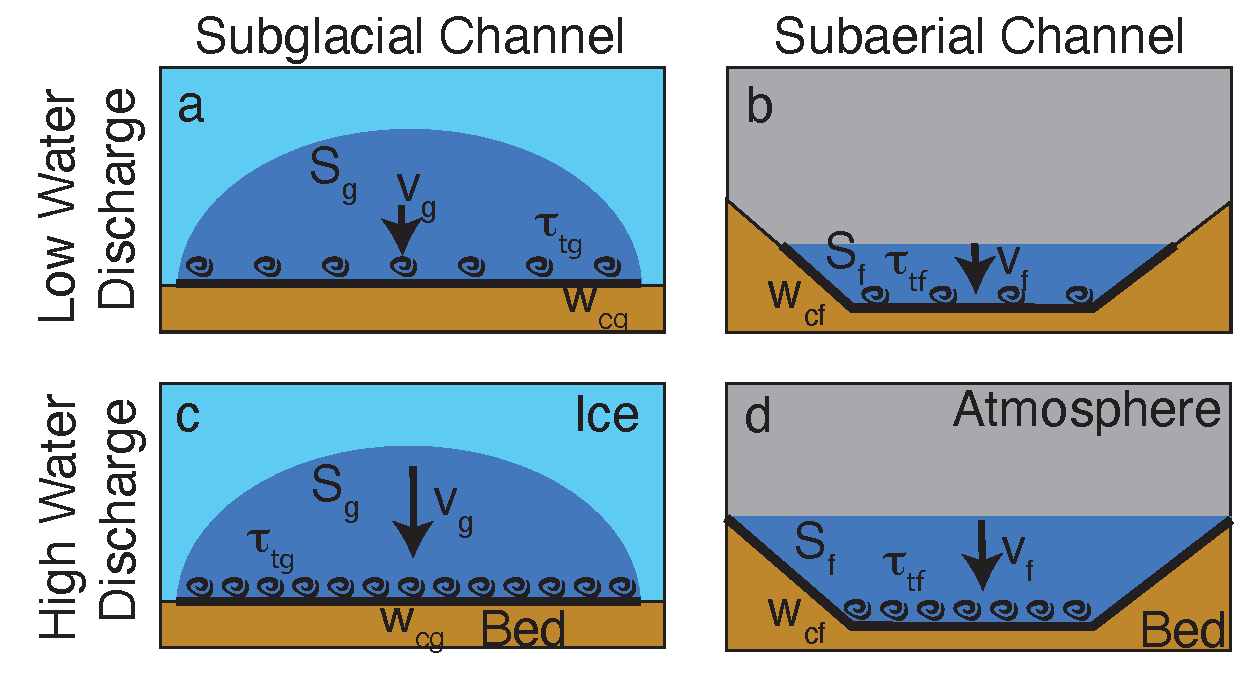
\includegraphics[width=0.65\linewidth]{Cartoon.pdf}
      \caption{Cartoon of the situation with various parameters. Water velocity magnitude in the subglacial, $v_g$, and subaerial, $v_f$, systems are shown by arrow length. $S_g$ and $S_f$ represent the cross-sectional area in subglacial and subaerial channels. The subglacial channel widths $w_{cg}$ remain steady, while the subaerial channel widths evolve $w_{cf}$, denoted by the thick black line. Shear stress $\tau$ is responsible for the mobilization of sediment and increases with the number of makers at the channel bed. 
        Note that in the subaerial channel parameterization, rectangular channel shapes are implemented (Section~\ref{sect:fluv}).} 
      \label{fig:cartoon}
    \end{figure}
  \end{center}


  
  \section{Methods}
  \label{sect:meth}
    Parameterizations below represent relationships amongst water discharge, subglacial water velocity, and channel geometry in both subaerial and subglacial channels (Table \ref{table:vpm}).
  Because sediment transport largely depends on shear stress applied by water flow \citep{shields1936}, both parameterizations calculate this value and integrate  it across the channel bed (Figure \ref{fig:cartoon}).
  The evaluation of shear stress omits a grain size parameter and, thus, leaves open the selection of a sediment transport relationship  \citep[e.g.][]{shields1936,meyer1948} to  calculate sediment transport capacity.
  As a result, relative relationships in shear stress, as opposed to sediment transport capacity, are examined.

  \begin{table}[H]
    \centering
    \caption{Variables, parameters, and constants }
    \begin{tabular}{ l  c  c c }
      Name &Symbol&  Value&Units \\ \hline
      \textbf{Variables}  & & & \\
      Channel hydraulic diameter (glacier, subaerial) &  $D_{hg},\,D_{hf}$&  & $\mathrm{m}$     \\
      Width of channel floor (glacial, subaerial) & $w_{cg},w_{cf}$&  & $\mathrm{m}$     \\
      Channel cross-sectional area (glacier, subaerial) &  $S_g, S_f$& & $\mathrm{m^2}$     \\
      Water discharge (instantaneous) & $Q_w$& & $\mathrm{m^{3}\,s^{-1}}$ \\
      Representative water discharge & $Q_{w}^*$& & $\mathrm{m^{3}\,s^{-1}}$ \\
      Representative hydraulic gradient  &$\Psi^*$ & & $\mathrm{Pa\, m^{-1}}$\\
      Water velocity (glacier, subaerial)  & $v_g,\,v_{f}$& & $\mathrm{m\,s^{-1}}$ \\
      Shear stress (glacier, subaerial) & $\tau_g,\,\tau_f$&& $\mathrm{Pa \, m^{-1}}$ \\
      Width-integrated shear-stress (glacier, subaerial) & $\tau_{tg},\, \tau_{tf}$&& $\mathrm{Pa \, m^{-1}}$ \\
      Reynolds number &$R_e$& & $\mathrm{(-)}$\\
      Variable &$\Gamma$&&$\mathrm{(-)}$\\
      Variability of a variable ($\Gamma$) &$\chi$& &$\mathrm{(-)}$\\
           &&&\\
      
      \textbf{Parameters and Constants}  & & &\\
      Gravitational constant&$g$& $-9.81$&$\mathrm{m\,s^{-2}}$\\
      Density of water & $\rho_w$& $1000$ & $\mathrm{kg\,m^{-3}}$ \\
      Density of ice & $\rho_i$& $900$ & $\mathrm{kg\,m^{-3}}$ \\
      Kinematic viscosity of water &$\nu$& $10^{-4}$& $\mathrm{m^2\,s^{-1}}$\\
      Hooke angle of channel & $\beta$ & $\frac{\pi}{2}$ & \unit{rad}\\
      Flotation fraction & $f_f$&$0.7$& $\mathrm{(-)}$\\
      Friction factor (glacier) & $f_r$ & $4$ & $\mathrm{(-)}$ \\
      Friction factor (subaerial) & $f_p$ & $3$ & $\mathrm{(-)}$\\
      Gradient of glacier surface & $\frac{\partial z_{sg}}{\partial x}$ &$0.25$& $\mathrm{(-)}$\\
      Gradient of channel bed (subaerial) &$\frac{\partial z_c}{\partial x}$ &$0.05$& $\mathrm{(-)}$\\
      Subaerial channel factor & $k$ &$3$ & $\mathrm{s\,m^{-2}}$\\
      Channel geometry exponent &$e$& $\frac{1}{2}$&$\mathrm{(-)}$ \\
      \hline
    \end{tabular}
    \label{table:vpm}
  \end{table}
  
  \subsection{Subglacial channel  parameterization}
  \label{sect:sub_mode}
  To evaluate the shear stress of water flowing across sediments below a glacier, the subglacial channel parameterization evaluates the channel geometry and the velocity of the flowing water.
  To accomplish this, the hydraulics model presented in \citet{delaney2019} is used.
  
  Here, it is assumed that the water is transported through subglacial channels \citep[Figure~\ref{fig:cartoon}; ][]{rothlisberger1972}, and that the channel  and geometry will respond to a representative water discharge over a certain time period $Q_{w}^*$, using the Darcy-Weisbach formulation for water-flow through a pipe  \citep[e.g.][]{rothlisberger1972,clarke2003,werder2013}.
  Thus, the hydraulic diameter of the subglacial channel, $D_h$, responds to a representative water discharge, $Q_{w}^*$, and a representative gradient of the hydraulic potential, $\Psi^*$ such that:
  \begin{linenomath*}
    \begin{equation}
      \label{eq:DW}
      D_h = \big(s\, f_r\,\rho_w\, \frac{Q_w^{*\,2}}{\Psi^*}\big)^{\frac{1}{5}}~~.
    \end{equation}
  \end{linenomath*}
  % 
  The representative hydraulic gradient is based upon the pressurized flow in Equation~\ref{eq:DW},
  \begin{equation}
    \label{eq:psi}
    \Psi^*= f_f \,  \rho_i \, g (\frac{\partial  z_{sg}}{\partial x} - \frac{\partial z_c}{\partial x}) +  \rho_i \, g \, \frac{\partial z_c}{\partial x},
  \end{equation}
  % 
  \noindent
  where, $f_f$ is the flotation fraction, $\rho_i$ is density of ice $\frac{\partial z_{sg}}{\partial x}$ is the surface slope of the glacier and $\frac{\partial z_c}{\partial x}$ is the glacier bed slope.
  
  In Equation~\ref{eq:DW}, $f_r$ is the Darcy-Weisbach friction factor and $\rho_w$ is the density of water (Table \ref{table:vpm}). $s$ is a factor accounting for channel geometry \citep{hooke1990}, calculated as:
  \begin{equation}
    \label{eq:Hf}
    s = \frac{2\,(\beta -\sin \beta)^2}{(\frac{\beta}{2}\,+\,\sin \frac{\beta}{2})^4},
  \end{equation}
  where $\beta$ is the central angle of the circular segment that comprises the channel (the so-called Hooke angle). Note that $\beta =\pi$ corresponds to a semi-circle and
  smaller values of $\beta$ result in shallow, wide channels. 
  The width of the flat channel floor $w_c$, given angle $beta$ is 
  \begin{equation}
    \label{eq:dh2wc}
    w_{cg} = 2  \sin \frac{\beta}{2} \sqrt{\frac{2\, S}{\beta -\sin \beta}},
  \end{equation}
  % 
  where $S$ is the cross-sectional area of the channel given by
  \begin{equation}
    \label{eq:dh2S}
    S_g =  \frac{D_h^2}{2}~ \frac{\Big(\frac{\beta}{2} \,+ \, \sin \frac{\beta}{2}\Big)^2  }{\beta\,-\,\sin \beta}.
  \end{equation}
  
  The shear stress, $\tau$, between the water and the channel bed is determined through the Darcy-Weisbach formulation
  \begin{equation}
    \label{eq:tau}
    \tau_g=\frac{1}{8}\,f_r\,\rho_w\,v_g^2,
  \end{equation}
  % 
  where  the water velocity $v_g$ is $v_g = \frac{Q_w}{S_g}$.
  Here, $Q_w$ represents the instantaneous water discharge, rather than $Q_w^*$, which is used to evaluate the channel geometry.
  With this formulation, the processes in an R-channel, through which water flows subglacially, can be represented algebraically \citep{rothlisberger1972,delaney2019}.
  
    Width integrated shear stress is represented as $\tau_{tg}=w_{cg}\,\tau_g $.
  
  \subsection{Subaerial channel  parameterization}
  \label{sect:fluv}
  
  To parameterize the shear stress of water flowing across sediments in the subaerial channel,  the hydraulics parameterization presented in \citet{tucker1997} is implemented.
  Here, it is assumed that there is a conservation of mass and a sufficiently wide channel so that the hydraulic radius is consistent with flow depth, uniform flow, and the Darcy-Weisbach relationship.
  The shear stress $\tau_f$ at the river bed is represented as
  \begin{linenomath*}
    \begin{equation}
      \label{eq:DW_tau}
      \tau_f=\frac{\rho_w\,g^{\frac{2}{3}}\,f_p^{\frac{1}{3}}}{2}\, \Big(\frac{Q_w}{w_{cf}} \Big)^{\frac{2}{3}} \,\frac{\partial z_c}{\partial x}^{\frac{2}{3}},
    \end{equation}
  \end{linenomath*}
  where $\frac{\partial z_c}{\partial x}$ is the channel slope, and $f_p$ is the friction factor for subaerial systems.
  Channel width $w_{cf}$ is 
  \begin{equation}
    \label{eq:wcf}
    w_{cf} = k \, Q_w^e,
  \end{equation}
  % 
  where $k$ is a constant and $e$ is an exponent commonly equal to $\frac{1}{2}$ \citep{leopold1953}.
  Cross-sectional area, $ S_f$, is 
  \begin{equation}
    \label{eq:Sf}
    S_f = \frac{Q_w}{v_f},
  \end{equation}
  % 
  where $v_f$ is water velocity, given by rearranging Equation \ref{eq:tau} as
  \begin{equation}
    \label{eq:vf}
    v_f = \sqrt{\frac{8\,\tau_f}{f_p\,\rho_w}}.
  \end{equation}
  % 
  As in Section~\ref{sect:sub_mode}, the width integrated shear stress is $\tau_{tf}=w_{cf}\,\tau_f$.
  Hydraulic diameter of the channel is given by $D_{hf} = \frac{4\,w_{cf}\,d}{2\,d+w_{cf}}$, with flow depth $d$ determined from knowledge of $S_f$ and $w_{cf}$ in a rectangular channel.
  
  \subsection{Implementation}
  
  The formulation of the glacial system (Section~\ref{sect:sub_mode}) requires inputs of the hydraulic gradient (Equation \ref{eq:psi}; $\frac{\partial z_{sg}}{\partial x}$, $\frac{\partial z_{c}}{\partial x}$), water discharge, $Q_w$ representative water discharge, $Q_w^*$,  Hooke angle (Equation~\ref{eq:Hf}; $\beta$), and friction factor (Equation~\ref{eq:DW}; $f_r$).

  
  In the subaerial system, the water is not pressurized, so only the bed slope, $\frac{\partial z_c}{\partial x}$, is needed in Equation~\ref{eq:DW_tau}. The friction factor, $f_f$, and channel shape factor, $k$, are assigned such that they produce reasonable values for water velocity and channel width  (Section~\ref{sect:fluv}).
  
  The Reynolds number $R_e$, which gives an evaluation of the degree of turbulence of the water, is given as 
  \begin{equation}
    \label{eq:re}
    R_e\,=\, v \,\frac{D_h}{\nu},
  \end{equation}
  % 
  \noindent where $\nu$ is the kinematic viscosity of water, and  $v$ is velocity of water, $v_g$ or $v_f$.
  
  The variance $ \chi$ of a variable $\Gamma$ is given by 
  \begin{equation}
    \label{eq:var}
    \chi(\Gamma) \,=\, 1 - \frac{\mathrm{min}(\Gamma)}{\mathrm{max}(\Gamma)}\,\,.
  \end{equation}
  % 
  \noindent Below we examine variables, $\Gamma$, as water discharge ($Q_w$) water velocity ($v_g$, $v_f$), shear stress ($\tau_g$, $\tau_f$), and integrated shear stress ($\tau_{tg}$, $\tau_{tf}$) with the purpose of evaluating total shear stress across the glacier bed.
  
  
  \section{Results}
  Initially, both parameterizations are forced with a water discharge ($Q_w$) varying between $8$ and $16$ \,\unit{m}$^{3}$\,\unit{s}$^{-1}$, to represent a range of sediment transport conditions, for instance over diurnal fluctuation in water discharge. The subaerial channel width factor $k$ is $3$\,\unit{m}$^{2}$\,\unit{s}$^{-1}$, and the Hooke angle $\beta$ is $\frac{\pi}{2}$.
  Values of Hooke angle $\beta$ and subglacial friction factor $f_r$ are chosen so that they produce reasonable values of water velocity ($0.6- 1.2$\,\unit{m}\,\unit{s}$^{-1}$) in accordance with measurements made through dye-tracing experiments to examine subglacial hydraulic conditions \citep[Section~\ref{sect:sub_mode}, Figure~\ref{fig:model_outs}; e.g.][]{werder2010}.
  The subglacial representative water discharge ($Q_w^*$; Equation~\ref{eq:DW}) of $12$\,\unit{m}$^{3}$\,\unit{s}$^{-1}$ is applied to establish the hydraulic diameter and shape of the channel.
  
  \begin{center}
    \begin{figure}[H]
      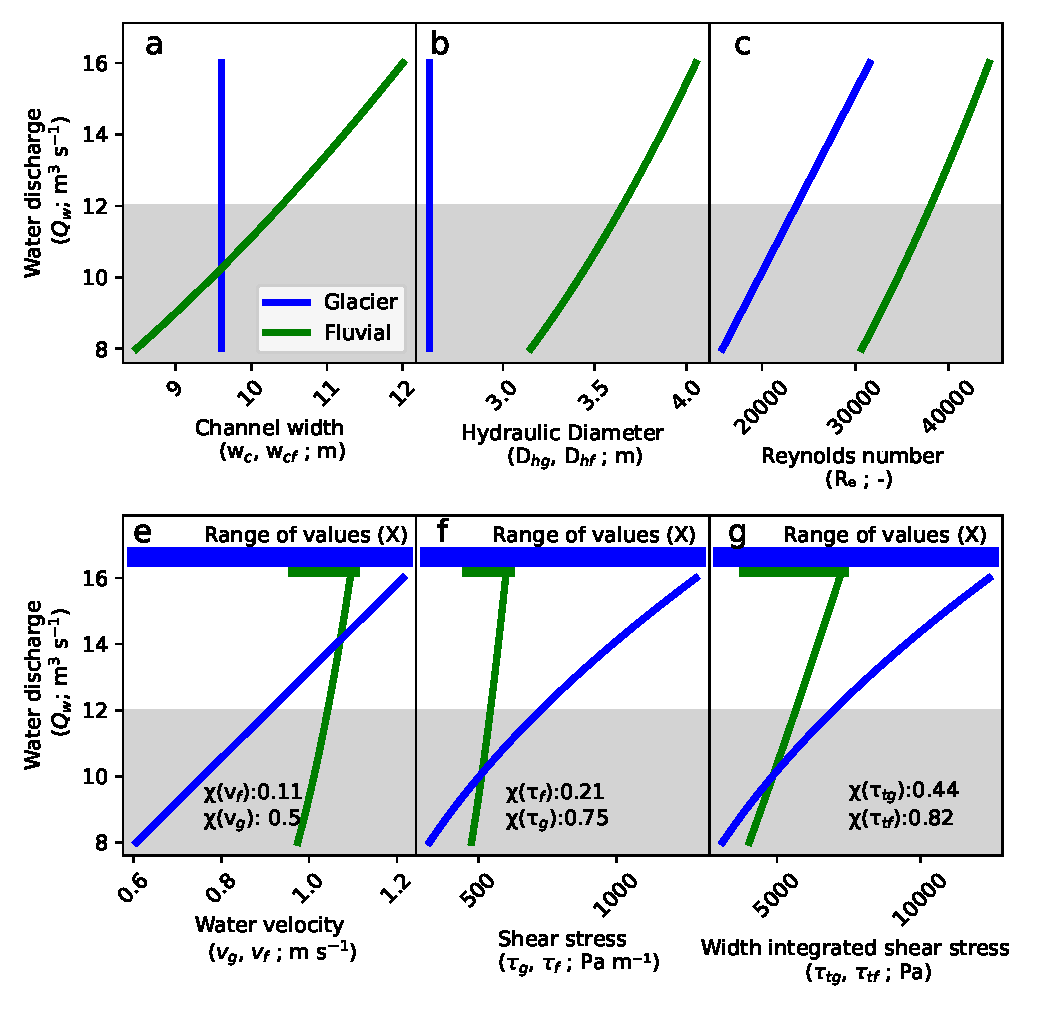
\includegraphics[width=0.7\linewidth]{model_outputs.pdf}
      \caption{Response of channel width (a), hydraulic diameter (b),  Reynolds number  (c),  water velocity (d), shear-stress (e), and width-integrated shear-stress (f)  to different water discharge values. The glacial system is in blue and the subaerial system is in green.  Horizontal bars in d, e, and f represent the range of values in the  output. Gray space represents water discharge below the mean value. }
      \label{fig:model_outs}
    \end{figure}
  \end{center}
  
  Across the hydrological forcing, variable water discharge results in a substantial increase in the range of water velocities in the glacial system compared to the subaerial system (Figure~\ref{fig:model_outs}).
  While water velocity in the glacier system varies by  $0.5$ (Equation~\ref{eq:var}) over the discharge values, in the subaerial system the water velocity only varies by $0.11$.
  Similarly, shear stress at the glacier bed varies by $0.75$ across the range of water discharge values, whereas shear stress across the subaerial system varies by roughly $0.21$. This increased variability  in shear stress between the two systems occurs as the water velocity is raised to the power of $2$ in Equation~\ref{eq:tau}. 
  
  Changing channel geometry accommodates evolving water discharge in the subaerial system (Equation~\ref{eq:wcf}), whereas in the subglacial case, increased water flux can only be accommodated by an increase in velocity (Equation~\ref{eq:DW}).
  The range of values between width-integrated shear stress in the subaerial system increases to $0.44$, whereas, variability in the glacial system lies at $0.83$ (Figure~\ref{fig:range}).
  Indeed, the relative  difference in width-integrated shear stress is less between the subaerial and glacier cases, compared to the water velocity and shear stress outputs.
  The reduced variability in width-integrated shear stress results from the additional width across the subaerial channel that accommodates a portion of the sediment transport capacity.
  
  Next, the parameterizations are run $25,000$ times with randomly selected channel geometries ($k=(2,6)$, $\beta=(\frac{\pi}{10},\pi)$), friction factors ($f_i=(0.001,20)$, $f_p=(0.001,20)$) and water discharges (maximum and minimum values selected between $5$ to $500$ \,\mmma). $Q_w^*$ in Equation ~\ref{eq:DW} is determined as the midpoint in the water discharge range. Parameter combinations are only selected if their maximum and minimum velocities are between $0.2$ and $3$\,\unit{m}\,\unit{s}$^{-1}$, resulting in roughly $10,600$ adequate parameter combinations. 
  
  
  \begin{center}
    \begin{figure}[H]
      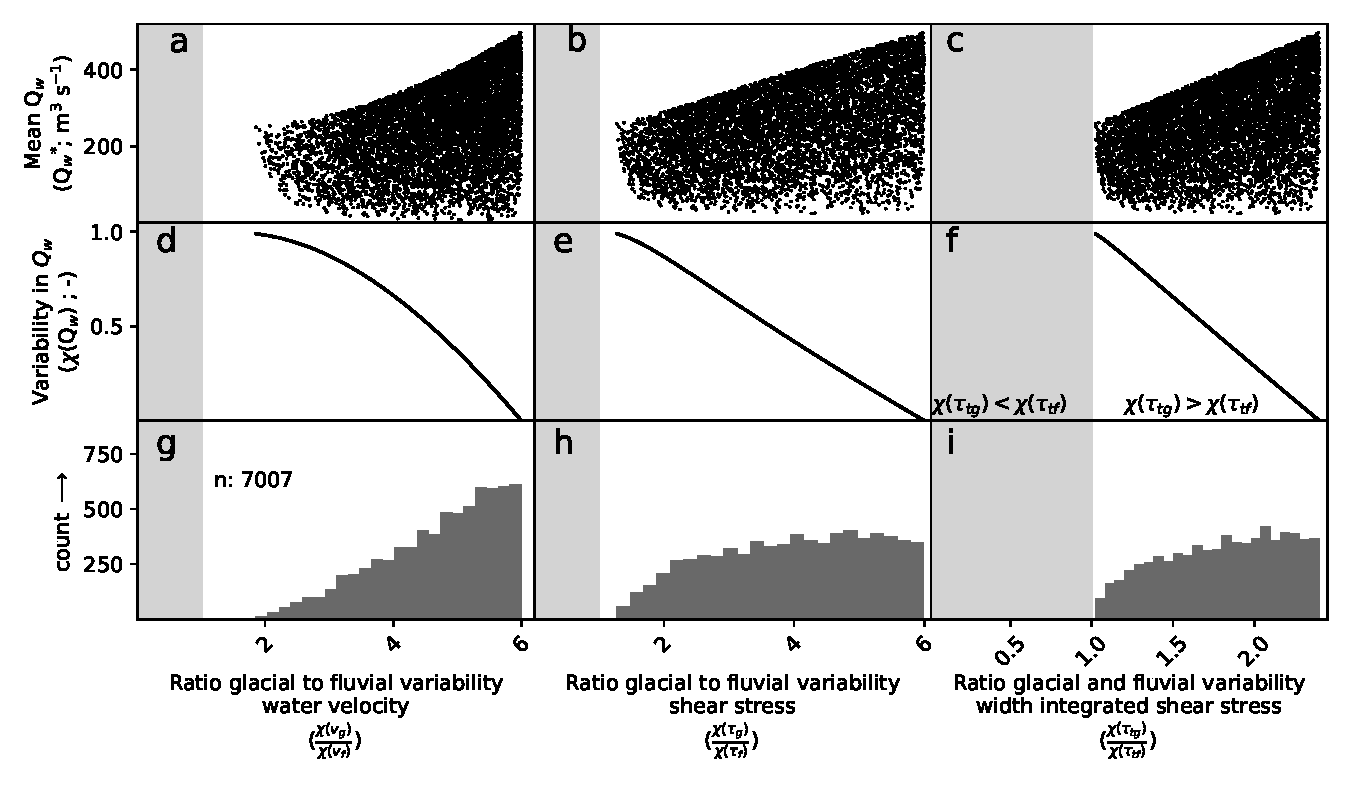
\includegraphics[width=0.7\linewidth]{multi_run.pdf}
      \caption{Ratio of range of water velocity, shear-stress, and width integrated shear-stress for glacial and subaerial systems in response to mean water discharge (a, b, c), and  variability in water discharge (d, e, f).  
        Range  $\chi$ for each variable is given in Equation~\ref{eq:var}. Values greater than $1$ shown in white space are parameter combinations that vary more in a subglacial  system.
        Histograms (g-i) show the frequency of relative variations across variables in the parameterization.}
      \label{fig:range}
    \end{figure}
  \end{center}
  
  Across the accepted model runs, variability in water velocity and shear stress remains substantially higher across the subglacial model compared to subaerial ones (Figure~\ref{fig:range}).
  Water velocity, shear stress, and width-integrated shear stress all have a variability ratio ($\frac{\chi(\Gamma_{g})}{\chi(\Gamma_f)}$) greater than $1$ in the subglacial  system compared to subaerial one (Figure~S \ref{fig:gammas}).
  
  The minimum ratio of  water velocity, $\frac{\chi(v_{g})}{\chi(v_{f})}$, and shear-stress, $\frac{\chi(\tau_{g})}{\chi(\tau_{f})}$, is around $2$, showing that these factors are substantially more variable in subglacial channels compared to subaerial ones (Figure~\ref{fig:range} g, h).
  The width integrated shear stress, $\frac{\chi(\tau_{tg})}{\chi( \tau_{tf})}$, spans between $1.02$ and $2.4$ because changing channel width accommodates some of the reduced shear stress variability in subaerial systems (Figure~\ref{fig:range} i).
  No runs experienced width integrated shear stress, $\frac{\chi(\tau_{tg})}{\chi( \tau_{tf})}$, less than $1$.
  
  Runs with the smallest variability in discharge ($\chi(Q_w)$) have the greatest variability in water velocity, shear stress, and width-integrated shear stress in subglacial systems compared to subaerial ones (Figure~\ref{fig:range} and S \ref{fig:gammas}).
  Yet, the greatest difference in the two systems at the smallest variations of water discharge still results in greater variability in the subglacial system compared to the subaerial one (Figure \ref{fig:range}). 

  
  \section{Discussion}
  \subsection{Assumptions}
  
 
  The subglacial parameterization assumes that subglacial water is pressurized, which is a commonly held assumption in subglacial hydrology, though observations suggest that this may not always be the case \citep[e.g.][]{gimbert2016}.
  The subglacial channel geometry need not be in equilibrium with the hydrological conditions for the water to remain pressurized.
  Yet the subglacial parameterization assumes that the channel geometry must vary minimally over the timescales of varying  water discharge \citep[e.g.][]{nanni2020}.
  
  In R-channel formulations, peaks in the hydrograph could cause additional opening of the conduit due to pressure melt, thus causing a decrease in velocity compared to the results here \citep{rothlisberger1972}.
  A similar effect could occur with creep closure of the subglacial channel at the hydrograph minima.
  Additionally, at high water pressures, glacier uplift and bed separation \citep{andrews2014} might modify the width of the subglacial channel. 

  Both subglacial and subaerial parameterizations here assume that the distribution of velocity and shear stress of water across the channel bed is homogeneous \citep[Section~\ref{sect:sub_mode}~and~\ref{sect:fluv}][]{yager2018}. 
  The subaerial parameterization assumes that sediment is transported across all channel widths, as opposed to large flows such as floods when much sediment transport occurs \citep{wolman1960}.
  As a result, the variability in the subaerial system across the range of discharge values could be underestimated in the parameterization (Figure~\ref{fig:range}).
 
  \subsection{Geomorphic Implications}
  \label{sect:GI}
  The relationship between water discharge variability and relative variability of the water velocity, shear stress, and width-integrated shear stress results from the fixed geometry in the glacier system and variable geometry in the subaerial system as they respond to changes in water discharge (Equations~\ref{eq:tau_t} and \ref{eq:v}).
  Increased variability in sediment transport capacity with respect to discharge has several implications for sediment transport in subglacial systems compared to subaerial ones.
  Shear stress is scaled to the $\frac{3}{2}$ power and relies on shear stress exceeding a threshold in sediment transport relationships  such as in \citet{meyer1948}.
  In the total sediment transport relationship \citet{engelund1967}, the shear stress is scaled to $\frac{5}{2}$ power.
  In both cases, the exponent greater than $1$ of shear stress in the sediment transport relationship magnifies the variability in sediment transport beyond the highly variable shear stress and width-integrated shear stress described above in subglacial environments (Figure~\ref{fig:model_outs}\, b and d; Figure~S~\ref{fig:gammas}).

  
  \subsubsection{Sediment transport below glaciers and at their margins}
  
  The response of sediment discharge caused by the greater variability in sediment transport in subglacial channels will be greatest in completely transport-limited regimes \citep[e.g.][]{kasmalkar2019}.
  In supply-limited systems, the changing sediment transport capacity (Figure~\ref{fig:model_outs}) would have a minimal effect on sediment discharge due to the absence of sediment available for transport \citep{delaney2019}.
  Yet, reaching the threshold of motion for sediment frequently, across a range of discharges,  may result in additional sediment transport and the tendency for glaciers to transport sediment in a supply-limited regime whereby sediment discharge scales with glacier sliding  \citep[e.g.][]{herman2015,koppes2015}.
  Sediment exhaustion by this process may also explain the dependence of sediment discharge from the Greenland Ice Sheet on basal shear stress, a proxy for bedrock erosion, as opposed to glacier melt \citep{overeem2017}.

  The effect of pressurized channel flow could be most pronounced during precipitation or flood events when subglacial conduits have not adapted to the water discharge flowing through them, resulting in a large increase in sediment transport capacity and discharge \citep[e.g.][]{cowan1988,delaney2019}.
  Increased sediment discharge may result from changes to sediment access below the glacier, yet rapid increases in water velocity from water flowing through a small channel will cause a large increase in sediment transport capacity (Section~\ref{sect:sub_mode}).
  
  Increased variability in sediment transport may also impact sediment export from the subglacial environment into proglacial areas \citep[e.g.][]{delaney2017,perolo2018}.
  Here, velocities at the highest water discharges could generally decrease (Figure~\ref{fig:model_outs}, blue and green horizontal bars), in the transition of pressurized subglacial flow to subaerial open-channel flow as the water leaves the glacier. The decrease in water velocity potentially results in sediment deposition once sediment enters the proglacial area.
  Periodic sediment deposition in sediment deposition may even result in the transition between pressurized and subaerial flow below the glacier terminus \citep{perolo2018}, especially when cavity closure rates of the ice are slow \citep{egli2021b}.
  
  In large catchments and further downstream of proglacial margins, water discharge is generally less variable than at the tops of catchments, where glaciers lie in alpine settings \citep[c.f.][]{swift2005,riihimaki2005,costa2017,vanas2017}.
  Here, external hydrological factors further downstream of glaciers could result in smaller variations in sediment transport capacity in many subaerial systems compared to subglacial ones.

  The parameterization here shows that the smallest variability in water discharge has the largest difference in relative variability in sediment transport metrics (Figure~\ref{fig:range}\, d,\,e,\,f).
  At locations such as the Greenland Ice Sheet, smaller diurnal variations in water discharge compared to many alpine catchments \citep[c.f.][]{swift2005,riihimaki2005,vanas2017,hasholt2018}.
  Therefore, the variability in sediment transport capacity in the transition from the ice sheet to the proglacial river could be more dramatic in Greenland than in alpine systems as water leaves the glacier and moves downstream.
  Thus the disparity in sediment transport capacity between the subglacial and subaerial systems could be most pronounced in larger catchments, potentially resulting in temporally mismatched periods between when glaciers introduce sediment to these river systems  and when the river mobilizes it (Figures~\ref{fig:model_outs}~ and~\ref{fig:range}).
  
  
  \subsubsection{Records of sediment discharge  from glaciers}
  
  Large variations in sediment transport capacity below glaciers may result in sediment mobilization and deposition processes in close spatial and temporal proximity to each other below the glacier \citep{gimbert2016,perolo2018}.
  The rapid increase and decreases in sediment transport capacity over a diurnal cycle in a subglacial system may compound the variability already present in subaerial systems \citep{williams1989,jerolmack2010}.
  As a result, variations in sediment transport capacity could be responsible for the fluctuations in sediment discharge (``flushings'') from glaciers that are not attributed to variations in water discharge \citep[e.g.][]{richards2003,swift2021}.
  Aside from the sporadic nature of these events, the observed flushings could result from increases in water velocity resulting from reduced channel size, not water discharge, which increase sediment transport capacity.

  Additional processes and erosional hiatuses may further complicate signals of sediment discharge from glaciers in response to climate, compared to subaerial systems \citep{jansson2005,ganti2016}. 
  For instance, sediment expelled from a glacier in a transport-limited regime reacts, in addition to water discharge, to sediment discharge capacity defined by the thickness of the ice, controlling the closure of the channel, and the surface slope of the glacier, controlling water velocity \citep[Section~\ref{sect:sub_mode}; ] []{rothlisberger1972,shreve1972,delaney2022,stevens2022}.
  Conversely, sediment transport in most subaerial systems increases with water discharge and bed slope, with the bed slope, probably being more stable over yearly to century-scale time periods \citep[Section~\ref{sect:fluv}; e.g.][]{muller1968,whipple1999,wong2006,wickert2019}. 
   
  Records of sediment discharge have been used to establish the relationship, or lack thereof, between sediment discharge and climate in glacial systems \citep[e.g.][]{koppes2009a,willenbring2016,mariotti2021}.
  The variability in subglacial sediment transport capacity presented here applies most generally to short-time scales responsible for the size of subglacial channels.
  Yet, identifying climatic signals in sediment transport from transport-limited glaciers may require higher thresholds of climatic perturbation compared to subaerial systems \citep{tofelde2021}, in addition to the stochastic nature of erosion and deposition in fluvial environments \citep{castletort2003,jerolmack2010,romans2016}.
  For instance, sediment discharge records from two glaciers in the Swiss Alps show that $40$ to $50$\% of a season's sediment discharge occurs when water discharge is below the $75^{\mathrm{th}}$ quantile of the season \citep{delaney2018}, possibly in part because sediment transport capacity responds the size of the glacier conduit, in addition to water discharge (Section~\ref{sect:sub_mode}).
  This suggests that a larger  perturbation of water discharge might be needed to significantly alter the sediment discharge capacity from the glaciers compared to subaerial systems, to overcome the noise resulting from increased variability in sediment transport capacity.
Furthermore, if no sediment is available and the glacier is in a supply-limited case, then the sediment discharge record will also represent additional processes of bedrock erosion from sliding and water pressure variations  \citep{iverson2012,herman2015}.

 
  \section{Conclusions}
  Contrary to subaerial channels that can alter their channel width and water velocity in response to changing water discharge,
   pressurized subglacial channels accommodate changing water discharge by altering water velocity and shear stress, upon which sediment transport depends.
  This occurs because the size of subglacial channels evolves slowly compared to variations in water discharge.
 
  Parameterizations of subglacial and subaerial water flow show that subglacial systems exhibit increased variability in sediment transport capacity as they respond  to changes in water discharge.
  The variability in sediment transport capacity is reduced when the evolving channel width is accounted for in subaerial systems.
  Even so, variability in sediment transport capacity across a channel's width is consistently higher in subglacial channels, compared to subaerial ones.
  
  These different characteristics between glacial and subaerial channels show that records of sediment transport downstream of glaciers capture both subglacial and subaerial processes together.
  Such processes might be particularly relevant at glacier margins, where water transitions from pressurized subglacial flow to open-channel subaerial flow.
  The inconsistent response of sediment transport in subglacial and subaerial systems to changing water discharge could add uncertainty in evaluating  sediment transport signals in subglacial systems.
  In addition, the subglacial parameterization shows that sediment transport capacity in glacier systems responds to a large number of factors such as channel size, ice thickness, and glacier surface slope, which may react to climate forcing differently than water discharge alone. 
  The differences in subglacial and subaerial channels' response to changing hydrology should be considered when examining sediment transport processes in glacierized catchments.
  
  \section{Acknowledgments}
  
  I was funded by SNSF Project No. PZ00P2\_202024.
  The julia code used herein is included in the supplementary material.
  
  
\end{spacing}

\bibliographystyle{apalike}
\bibliography{Paperlib.bib}


\section{Supplement}

\renewcommand{\figurename}{Figure S}
\setcounter{figure}{0}

\begin{center}
  \begin{figure}[H]
    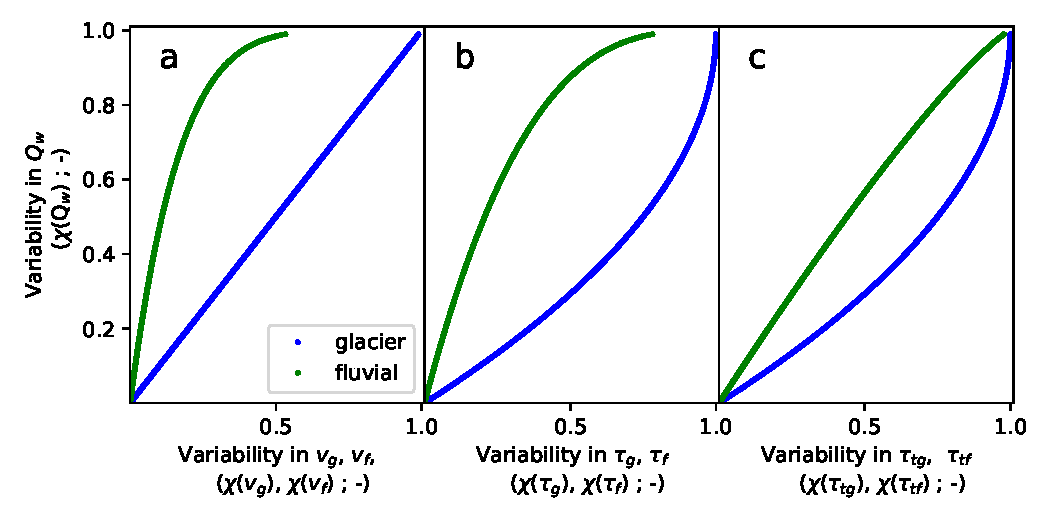
\includegraphics[width=0.7\linewidth]{multi_run_vars.pdf}
    \caption{Variability $\chi$ in velocity ($v_g$, $v_f$; a) shear stress ($\tau_g$, $\tau_f$; b) and width-integrated shear stress ($\tau_{tg}$, $\tau_{tf}$; c)  in glacial and subaerial systems. Across the parameter space in Figure~\ref{fig:range}. }
    \label{fig:gammas}
  \end{figure}
\end{center}




\end{document}

%%% Local Variables:
%%% mode: latex
%%% TeX-master: t
%%% End:

% LocalWords:  pre todo phillips CVODE decadal refreezing Mauro eq%  LocalWords:  dQs
% LocalWords:  dx ms ca DF Hm meltwater Griessee gridded ehrbar ng
% LocalWords:  koppes costa bendixen delaney herman hallet creyts ian
% LocalWords:  farinotti stott rickenman delaney2019 plagerized
% LocalWords:  fischer zekollari clarke raymond larour delaneyinprep
% LocalWords:  guillon exner wolman engelund Weisbach

